\documentclass[oneside,11pt]{starlink}


% ------------------------------------------------------------------------
% starlink set up
%\title{SSN/79}
\stardoccategory  {Starlink System Notes}
\stardocinitials  {SSN}
\stardoccopyright{Copyright \copyright\ 2015 University of British Columbia}
\stardocnumber    {79.1}
\stardocsource    {ssn\thestardocnumber}
\stardocauthors   {Gaelen Marsden}
\stardocdate      {8th January 2015}
\stardoctitle     {Further parallelization of iteratemap with MPI}
\stardocversion   {Version 0.1}
%%\stardocmanual    {User's Guide}
\stardocabstract  {
  This document describes how to extend the parallelization of the
  iterative makemap method for use on a distributed-memory cluster using
  the MPI. A prototype demonstrating the algorithm can be found at
  \url{github.com/CCATObservatory/mpi-mapmaker-test}.
}
%%\starfunders{University of British Columbia \& the Science \& Technology Facilities Council}
%%\startitlepic{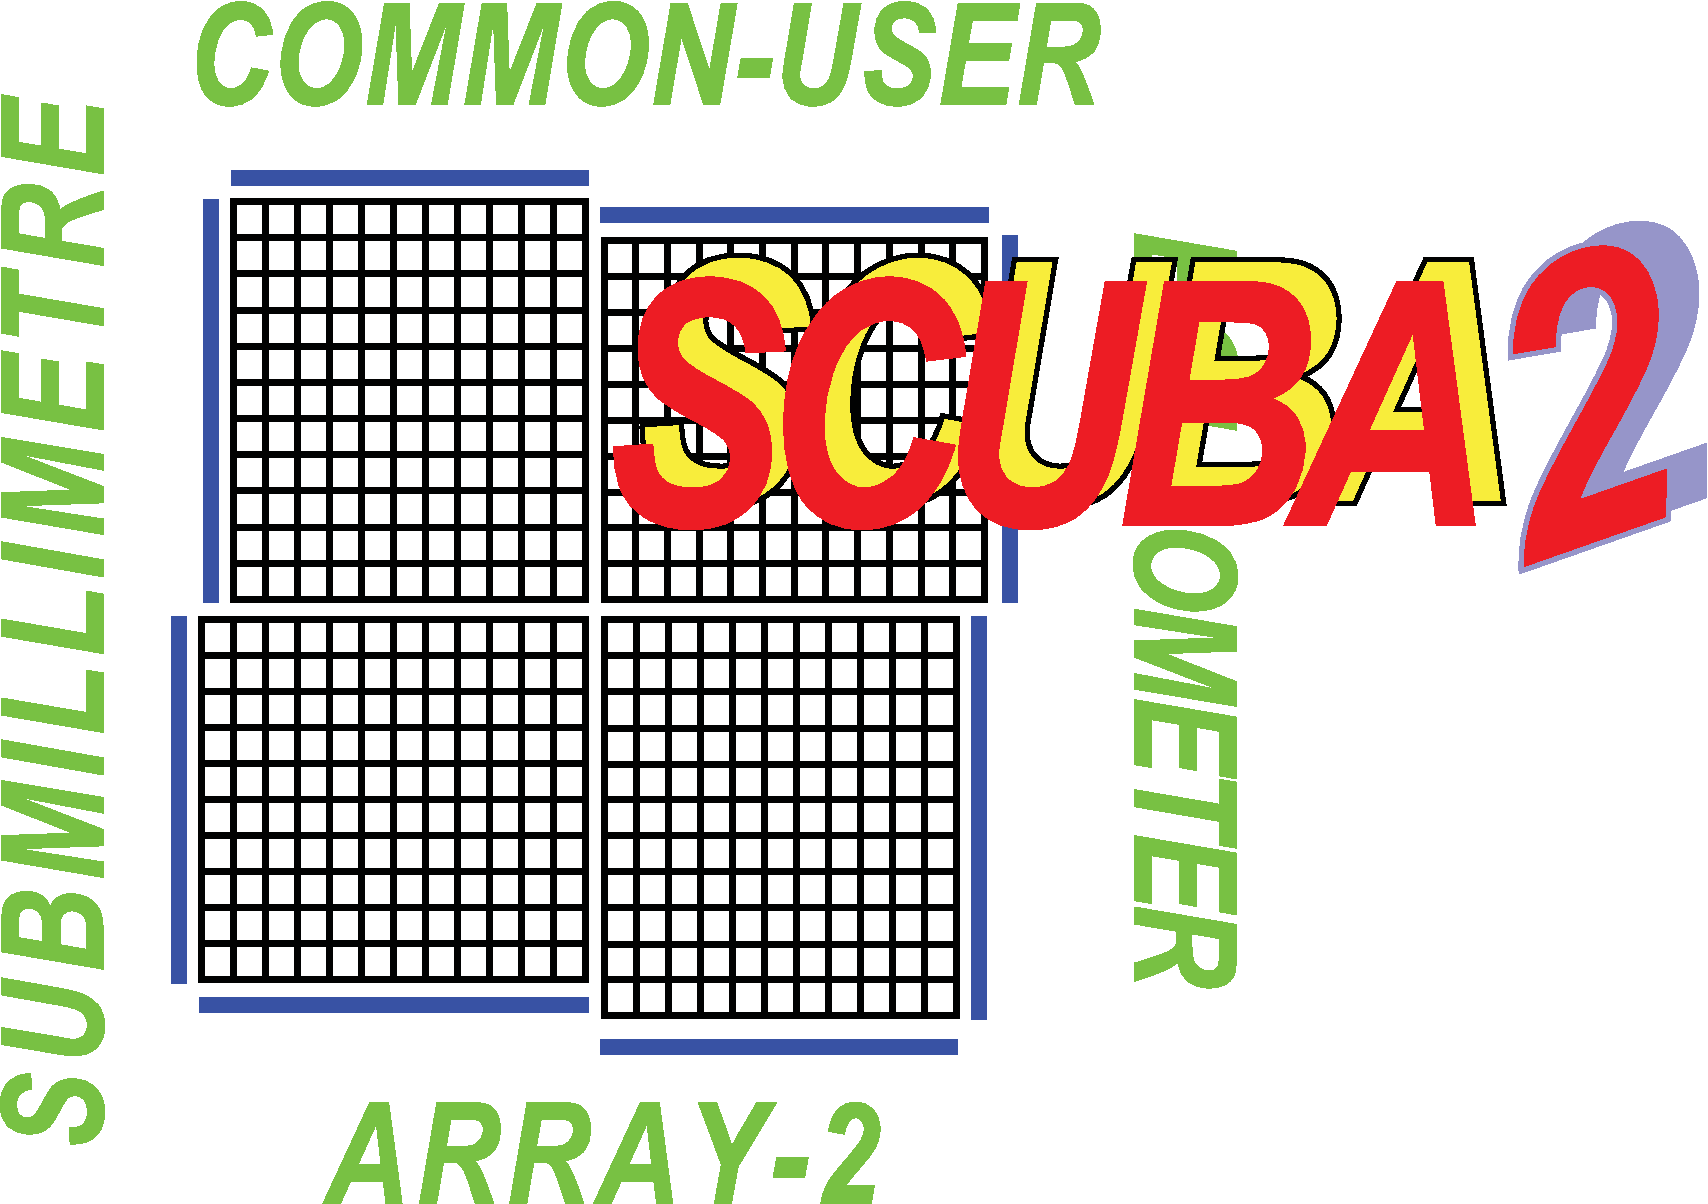
\includegraphics[width=0.55\textwidth]{sun258_logo}}



\begin{document}

\scfrontmatter

%%%%%%%%%%%%%%%%%%%%%%%%%%%%%%%%%%%%%%%%%%%%%%%%%%%%%%%%%%%%%%%%%%%%%%%%%
\section{\xlabel{introduction}Introduction\label{se:intro}}
%%%%%%%%%%%%%%%%%%%%%%%%%%%%%%%%%%%%%%%%%%%%%%%%%%%%%%%%%%%%%%%%%%%%%%%%%

The iterative map-maker developed for \SMURF\ is a sophisticated
algorithm that is able to reduce the large amounts of data collected
by SCUBA-2 in a reasonable amount of time. The algorithm measures and
removes correlated noise by iteratively solving for sources of noise
along with the sky signal. This is much less computationally intensive
than a full generalized least squares solution
(e.g.\ \cite{patanchon2008}), which requires careful measurements of
noise auto- and cross-power spectra and inversion of very large
matrices. Due to the iterative nature of the algorithm, however, the
full data set must be accessed repeatedly. Since the data rate is high
(10s of GB per hour of observation), reading the full data set (often
many hours) from disk is slow. Re-reading the data on every iteration
takes a considerable amount of time, so it is desirable to keep the
data in memory once it has been read in the first time. This limits
the amount of data that can be reduced at a time. Longer observations
with data sizes larger than than the available memory must be reduced
in chunks and combined after the fact, if caching and re-reading the
data is to be avoided.

The next generation of submillitre instruments, such as SWCam
\cite{stacey2014}, the short-wavelength camera for CCAT
\cite{jenness2014}, will have 10 times as many detector elements as
SCUBA-2 and will be sampled at a rate of ${\sim} 1$\,kHz, compared to
SCUBA-2's ${\sim} 200$\,Hz. This increase in data volume by a factor
of ${\sim} 50$ presents a serious problem for data reduction, both
in terms of memory usage and processing time. Several approaches have
been considered to account for this large increase in data volume:

\begin{enumerate}

\item High-pass filter the time-streams to suppress low-frequency
  correlated noise. If the detectors' filtered noise power spectra are
  reasonably flat and uncorrelated, the map-making problem becomes one
  of simply rebinning (averaging all samples that fall within a given
  sky pixel), requiring only one pass through the data. The high-pass
  filter limits the angular scales recovered by the mapping process,
  however; this is fine for maps consisting of only point sources, but
  when larger scales are important, this approach will not be
  sufficient.

\item Use machines with large amounts of memory and limit the length
  of observations that can be reduced in a single pass. CCAT and SWCam
  are still several years away, and one can expect increases in
  hardware speed and capacity in the intervening years. By simply
  scaling the run time and memory usage for reducing 15 minutes of
  SCUBA-2 data, we estimate that a 32-core machine with 2\,TB memory
  could reduce 15 minutes of SWCam data in about an hour
  \cite{marsden2014a}. Four such machines would therefore be needed to
  reduce the data as it is collected, and would be limited to small
  maps.

\item Write a parallel version of map-maker to run on a
  distributed-memory cluster of machines. The iterative algorithm is
  not trivially parallelizable, as each iteration and each model
  within each iteration must be calculated sequentially. The solution
  then is to parallelize each model calculation. This is also
  non-trivial, as some models require access to all detectors at each
  time slice (e.g.\ the common model model), some models require all
  time samples for each detector (e.g.\ the high-pass filter), and
  some require all samples (e.g.\ the astronomical model). We solve
  this problem by message-passing via MPI.\footnote{Message Passing
    Interface: a standard defining a set of routines to pass messages
    between processes.}

\end{enumerate}

The distibuted-memory parallelized version of the iterative map-maker
has been described elsewhere \cite{marsden2014b}, but in this document
we add more detail and discuss some practical considerations.

A note on terminology: a distributed-memory \textit{cluster\/}
consists of a number of connected \textit{nodes}. Each node may
consist of a number of \textit{processors\/} or cores. A single node
can support multithreaded parallelization using shared memory between
threads. The term \textit{process\/} refers to a single executable
that is run on a node; a process is able to spawn multiple threads to
take advantage of a multicore node. The term \textit{system\/} is used
to refer to the set of all processes involved in the calculation.

%%%%%%%%%%%%%%%%%%%%%%%%%%%%%%%%%%%%%%%%%%%%%%%%%%%%%%%%%%%%%%%%%%%%%%%%%
\section{\xlabel{algorithm}Parallel Algorithm\label{se:algorithm}}
%%%%%%%%%%%%%%%%%%%%%%%%%%%%%%%%%%%%%%%%%%%%%%%%%%%%%%%%%%%%%%%%%%%%%%%%%

The iterative map-making algorithm as implemented by \makemap\ is
described in detail in \cite{chapin2013}. Figure~\ref{fig:serial}
shows the overall flow of the algorithm. Data are read from disk,
prepocessing steps (such as calibration and spike detection) are
applied, and then a series of models is fit to the time-stream
residuals with the other best-fit models removed (initially
assuming all models are zero). This procedure is iterated until a
convergence criterion or criteria is reached.

\begin{figure}[ht]
\begin{center}
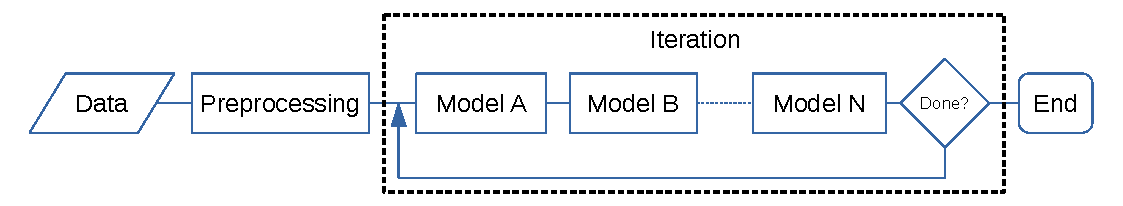
\includegraphics[width=\textwidth]{ssn79_serial_flowchart}
\caption[Serial flow chart]{The serial version of the iterative
  map-maker. The modules within the dashed box are part of the
  iteration loop, which is terminated when a convergence criterion or
  criteria is met.}
\label{fig:serial}
\end{center}
\end{figure}

In the distributed-memory parallel version, each process reads a
distinct chunk of data, applies the preprocessing steps, and proceeds
to calculate the models, as in the serial version. Each model is then
responsible for communication between processes to ensure that it is
properly fit to the full data set. See Figure~\ref{fig:parallel}.

\begin{figure}[ht]
\begin{center}
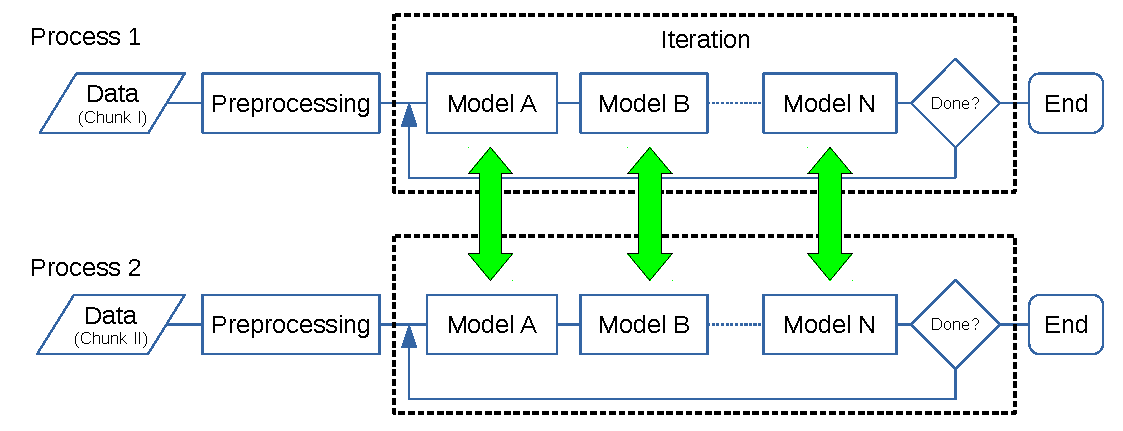
\includegraphics[width=\textwidth]{ssn79_parallel_flowchart}
\caption[Parallel flow chart]{The distributed-memory parallel version
  of the iterative map-maker is essentially $N_\mathrm{node}$
  map-makers running independently, except that communication between
  processes is required to calculate the models (represented by green
  arrows). Note that the termination condition (represented by
  ``Done?'' in the figure), which could be looking at the change in
  RMS of the residuals, also requires communication between
  processes.}
\label{fig:parallel}
\end{center}
\end{figure}

By breaking up the data set over $N_\mathrm{node}$ processes, we are
able to handle data sets much larger than can be done with a single
machine. Additionally, since the calculations are split up over many
nodes, the map-maker can in principle run much faster than the serial
version. The speed-up in run time is not simply $1/N_\mathrm{node}$,
however, due to the time required by the communication steps, which
can be significant. Also, since the model calculations proceed
sequentially, the system proceeds only as fast as the slowest
node. The scaling of run time with number of processes for a prototype
of this algorithm has been discussed elsewhere
(\cite{jenness2014,marsden2014b}).

We point out that \makemap\ is already multithreaded using pthreads
to take advantage of multi-core CPUs. We intend to implement the
distributed-memory parallelization while maintaining the
multithreading, as the shared-memory parallelization is much more
efficient since there is little communication overhead.

%%%%%%%%%%%%%%%%%%%%%%%%%%%%%%%%%%%%%%%%%%%%%%%%%%%%%%%%%%%%%%%%%%%%%%%%%
\section{\xlabel{models}Parallelizing the Models\label{se:models}}
%%%%%%%%%%%%%%%%%%%%%%%%%%%%%%%%%%%%%%%%%%%%%%%%%%%%%%%%%%%%%%%%%%%%%%%%%

The parallelization of the iterative map-maker is accomplished by the
individual model. Each model is responsible for ensuring that it is
fit to all applicable data and that the best-fit model is distributed
to all processes. There are three classes of models to consider; those
that require:

\begin{enumerate}
\item all time samples for each individual detector (e.g.\ high-pass
  filter)
\item all detector samples at each time slice (e.g.\ common mode)
\item some more-complicated division of the data set
  (e.g.\ astronomical signal, which could be solved by dividing the
  samples by region on the sky)
\end{enumerate}

We can choose the division of the data set between nodes to make one
of the model types easy to calculate, but not all of them. Because the
high-pass filter model performs FFTs on the detector time streams,
which we would hard to perform if an individual detector was spread
out across nodes, we decide to split the data between nodes so that
each process acts on the complete time streams for a number of
detectors.

The parallelization of the example models listed above are now described
in some detail to illustrate how the parallelization of the different
model-types is accomplished.

%%%%%%%%%%%%%%%%%%%%%%%%%%%%%%%%%%%%%%%%%%%%%%%%%%%%%%%%%%%%%%%%%%%%%%%%%
\subsection{High-pass Filter}
%%%%%%%%%%%%%%%%%%%%%%%%%%%%%%%%%%%%%%%%%%%%%%%%%%%%%%%%%%%%%%%%%%%%%%%%%

Figure~\ref{fig:serial_highpass} illustrates how the existing
multithreaded map-maker performs the convolutions necessary for the
high-pass filter model. Since each detector time-stream can be
processed independently, the detectors are divided into
$N_\mathrm{thread}$ chunks and each thread performs the convolution of
each detector with the filter and stores the result directly in a
shared-memory array.

\begin{figure}[ht]
\begin{center}
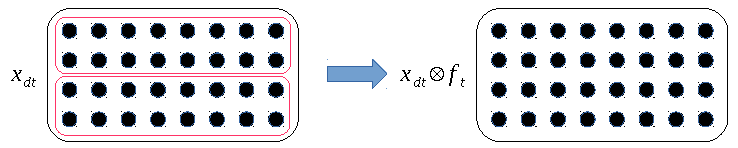
\includegraphics[width=0.5\textwidth]{ssn79_serial_highpass}
\caption[Serial High-pass Filter Model]{Illustration of the
  calculation of the high-pass filter model on four detectors with
  eight time-samples each, using two threads. The red outlines
  indicate how the data are chunked for processing by each thread.}
\label{fig:serial_highpass}
\end{center}
\end{figure}

With full detector time streams on each node, parallelizing the
high-pass filter model is trivial, as shown in
Figure~\ref{fig:parallel_highpass}. Each node is responsible for
$N_\mathrm{det} / N_\mathrm{node}$ detectors which are then further
split up for each thread. No communication between processes is
required.

\begin{figure}[ht]
\begin{center}
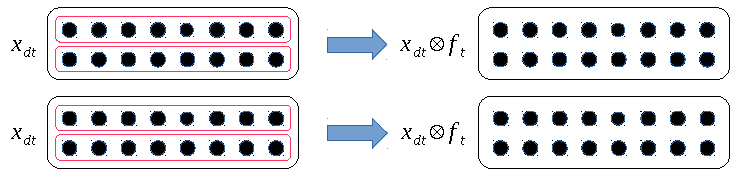
\includegraphics[width=0.5\textwidth]{ssn79_parallel_highpass}
\caption[Parallel High-pass Filter Model]{Parallel version of the
  high-pass filter model. Here we have two processes (represented by
  black outlines), each with two threads. The model is trivially
  parallelized, as each detector can be processed independently.}
\label{fig:parallel_highpass}
\end{center}
\end{figure}

%%%%%%%%%%%%%%%%%%%%%%%%%%%%%%%%%%%%%%%%%%%%%%%%%%%%%%%%%%%%%%%%%%%%%%%%%
\subsection{Commom-mode Model}
%%%%%%%%%%%%%%%%%%%%%%%%%%%%%%%%%%%%%%%%%%%%%%%%%%%%%%%%%%%%%%%%%%%%%%%%%

The calculation of the common-mode model is illustrated in
Figure~\ref{fig:serial_common}. The data are now chunked along the
detector dimension so that each thread calculates the average detector
value for each of a range of time slices. This is shown in the figure
as a two-step process:  the signal and number of samples are
accumulated into arrays, and then the accumulated sums are divided by
the number of samples. It is shown this way so that the generalization
to the parallel version is more clear.

\begin{figure}[ht]
\begin{center}
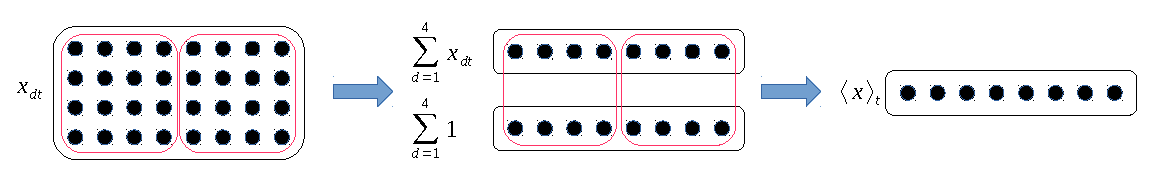
\includegraphics[width=0.8\textwidth]{ssn79_serial_common}
\caption[Serial Common-mode Model]{Illustration of the calculation of
  the common-mode model on a single node using two threads. The data
  are chunked along the detector axis so that each thread can
  calculate the common-mode signal (average value) at each time
  sample. The calculation of the average is shown in two steps: first
  the signal and number of detectors are accumulated at each time
  slice, then the average at each step is calculated. Note that it is
  simple to extend this to a weighted average by accumulating
  $w_\mathrm{dt} x_\mathrm{dt}$ and $w_\mathrm{dt}$ instead of
  $x_\mathrm{dt}$ and 1.}
\label{fig:serial_common}
\end{center}
\end{figure}

In the parallel version, a single process is not able to fully
calculate the model. Instead, each process accumulates the sums for
its set of detectors, then MPI communications are used to accumulate
the arrays across all processes. Each process can then perform the
final division of the accumulated arrays. The parallel version is
shown in Figure~\ref{fig:parallel_common}.

\begin{figure}[ht]
\begin{center}
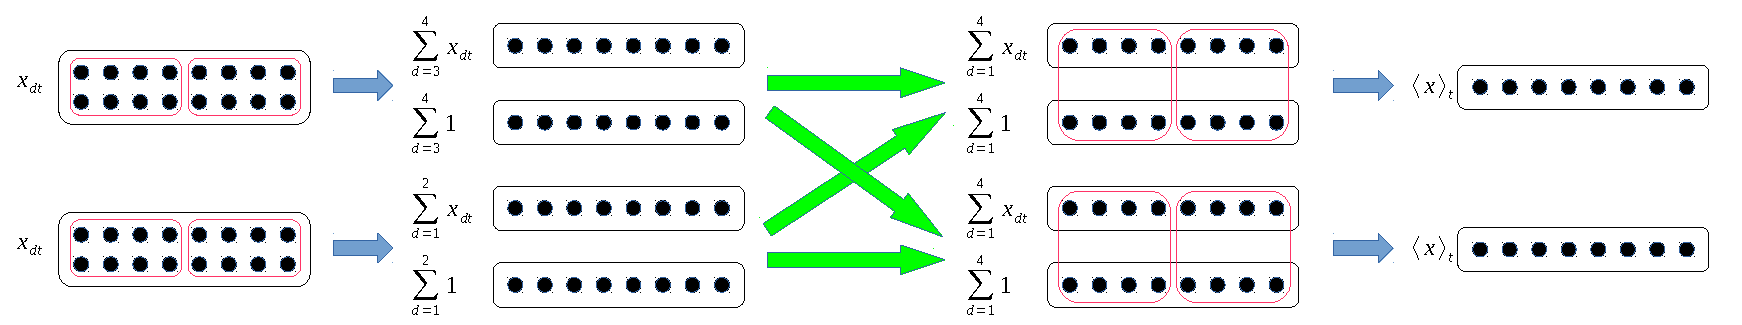
\includegraphics[width=\textwidth]{ssn79_parallel_common}
\caption[Parallel Common-mode Model]{Parallel version of the
  common-mode model. An extra commumincation step (represented by
  green arrows) is inserted, where the arrays are accumulated across
  all nodes. Multithreading is still used for parallelized calculation
  of the model.}
\label{fig:parallel_common}
\end{center}
\end{figure}

The code to perform this operation might look something like this:

\begin{verbatim}
for (idet=0; idet<ndet; idet++) {
  for (isamp=0; isamp<nsamp; isamp++) {
    signal[isamp] += data[idet*ndet+isamp];
    count[isamp] += 1;
  }
}

#if USE_MPI
MPI_Allreduce(MPI_IN_PLACE, signal, nsamp, MPI_DOUBLE, MPI_SUM, MPI_COMM_WORLD);
MPI_Allreduce(MPI_IN_PLACE, count, nsamp, MPI_DOUBLE, MPI_SUM, MPI_COMM_WORLD);
#endif

for (isamp=0; isamp<nsamp; isamp++) {
  signal[isamp] /= count[isamp];
}
\end{verbatim}

This program is run by each process, where \verb+ndet+ is the number
of detectors ``owned'' by the process, and is not restricted to be the
same in each process. The communications are performed by the MPI
command \verb+MPI_ALLreduce+, which performs the exact operation we
need: an array (\verb+signal+ and \verb+count+ in the examples above)
is combined across processes with a specified operation (here, we
specify ``sum'') and the result is returned in place to each
process. Following the communication step, each process calculates the
average for itself---this is quicker than having a single thread
calculate the average and then communicate the result. Also note that,
without the ``\verb+#if USE_MPI/#endif+'' clause, the code is
identical to what is calculated by the serial version.

%%%%%%%%%%%%%%%%%%%%%%%%%%%%%%%%%%%%%%%%%%%%%%%%%%%%%%%%%%%%%%%%%%%%%%%%%
\subsection{Astronomical Sky Model}
%%%%%%%%%%%%%%%%%%%%%%%%%%%%%%%%%%%%%%%%%%%%%%%%%%%%%%%%%%%%%%%%%%%%%%%%%

The astronomical sky model rebins the data time streams, after
subtraction of noise models, into a map of the sky, the end product of
the map-maker. The projection for detector/time sample to map pixel is
a complicated function depending on the focal plane layout and
telescope scan pattern, and thus the task cannot be easily subdivided
into a number of independent tasks in the same way that is done for
the filter and common-mode models. Instead, each thread in the
single-node version of the map-maker has its own copy of the map
arrays and accumulates a chunk of the data samples; the data could be
chunked either by detector or time sample. After each thread has
finished accumulating its samples, the accumulator arrays are combined
and the final division is performed.

The paralellization of this calculation is analogous to the
common-mode model; after the threaded accumulator arrays are combined,
the arrays are accumulated across nodes, again using
\verb+MPI_Allreduce+, and the divisions are performed by each process.

%%%%%%%%%%%%%%%%%%%%%%%%%%%%%%%%%%%%%%%%%%%%%%%%%%%%%%%%%%%%%%%%%%%%%%%%%
\subsection{Other Models}
%%%%%%%%%%%%%%%%%%%%%%%%%%%%%%%%%%%%%%%%%%%%%%%%%%%%%%%%%%%%%%%%%%%%%%%%%

Models other than the ones discussed above should fall within one of
the categories discussed above. Communication commands other than
\verb+MPI_Allreduce+ or operators other than \verb+MPI_SUM+ may be
needed for more complicated model-fitting.

%%%%%%%%%%%%%%%%%%%%%%%%%%%%%%%%%%%%%%%%%%%%%%%%%%%%%%%%%%%%%%%%%%%%%%%%%
\section{\xlabel{implementation}Implementation
  Details\label{se:implementation}}
%%%%%%%%%%%%%%%%%%%%%%%%%%%%%%%%%%%%%%%%%%%%%%%%%%%%%%%%%%%%%%%%%%%%%%%%%

It will take some work to take the parallel algorithm described here
and implemented in the prototype and apply it to \makemap. Some of the
issues that will have to be considered are listed:

\begin{itemize}

\item Do we need to dynamically determine the amount of memory on each
  node? \makemap\ measures the total available memory and decides how
  much data to process at one time based on the result. But in a
  typical cluster queueing system, one requests a specific amount of
  memory per node, so this step might not be needed.

\item A related question is how should the load be balanced? Do we
  allow for heterogenous clusters of nodes? One could imagine
  determining the available memory, number of processors and processor
  speed on each node and balance the data accordingly. But it would
  be much simpler to assume the method will only be run on homogeneous
  clusters and divide the data evenly between the nodes.

\item Communication is also needed any time a return status is
  checked, since if one process is going to abort, then whole system
  should abort. It should be sufficient to precede each status test
  with an \verb+MPI_Allreduce+ call on the status variable using the
  operator \verb+MPI_LOR+ (``logical or'').

\item For certain models it may be more efficient to consider
  communicators other than the default \verb+MPI_COMM_WORLD+, which
  consists of all processes in the system. For example, one might like
  to calculate the common mode on a per-array basis rather than a
  single mode for all detectors. If the detectors are split across
  nodes such each node has detectors belonging to only one array, a
  communicator can be created for each array (consisting of the nodes
  that contain data from that array), and then the same form
  of \verb+MPI_Allreduce+ can be used, with each node specifying the
  appropriate communicator. This type of sub-division could help with
  the communication overhead.

\end{itemize}


%%%%%%%%%%%%%%%%%%%%%%%%%%%%%%%%%%%%%%%%%%%%%%%%%%%%%%%%%%%%%%%%%%%%%%%%%
\begin{thebibliography}{}
\addcontentsline{toc}{section}{\protect\numberline{}References}
%%%%%%%%%%%%%%%%%%%%%%%%%%%%%%%%%%%%%%%%%%%%%%%%%%%%%%%%%%%%%%%%%%%%%%%%%

\bibitem{patanchon2008}
Patanchon~G.~P., et~al., 2008, ApJ, 681, 708

\bibitem{stacey2014}
Stacey~G., et~al., 2014, Proc.\ SPIE 9153, 915321

\bibitem{jenness2014}
Jenness~T., et~al., 2014, Proc.\ SPIE, 9152, 91522

\bibitem{marsden2014a}
Marsden~G., et~al., 2014, ASPC, 485, 399

\bibitem{marsden2014b}
Marsden~G., et~al., 2014, arXiv:1410.8416

\bibitem{chapin2013}
Chapin~E.~L., et~al., 2013, MNRAS, 430, 2545

\end{thebibliography}

\end{document}


